\chapter{Geophysics Interferometer (GIF)}
KAGRA is the only GW detector, which has a strainmeter to monitor the baseline length changes. The strainmeter is named Geophysics interferometer (GIF).

GIF is a laser interferometric strainmeter, which is developed by Earthquake Research Institute, University of Tokyo. The purpose of the strainmeter is observe the geophysical phenomena such as 


In this chapter, GIF is described.

\section{Overview}
Geophysics interferometer (GIF) is a $1500\,\mathrm{m}$ laser strainmeter constructed along the X-arm baseline of KAGRA. As shown in Fig.\ref{img:img402}, GIF is an asymmetric Michelson interferometer unlike KAGRA interferometer. Moreover, mirrors of the interferometer of GIF are fixed on the ground to monitor the baseline length changes directly. GIF is now only installed on the X-arm. GIF have been observing the baseline changes for almost 3 years.
\begin{figure}[h]
  \centering
  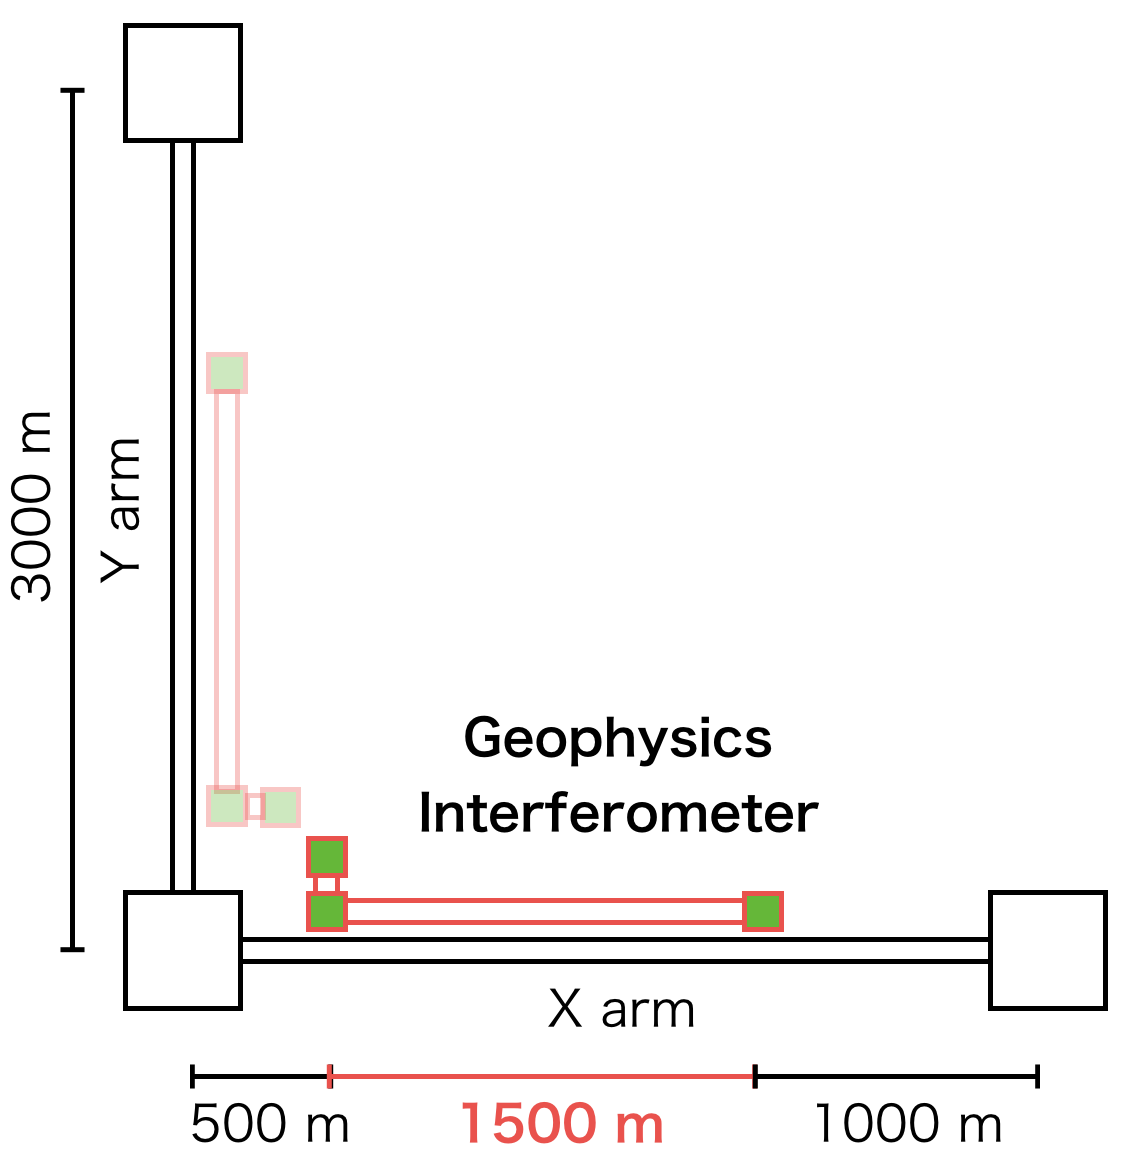
\includegraphics[width=6.5cm]{./img_chap4/img402.png}
  \caption{Location of geophysics interferometer (GIF). } \label{img:img402}
\end{figure}


\section{Working Principle}
Section \cref{sec:12} で述べたMichelson干渉計と同じであるので動作原理は同じであるが、GIFの場合、非対称Michelson干渉計なので周波数ノイズがひずみ計測の感度を制限する。

\subsection{Asymmetric Michelson Interferometer}
\begin{figure}[h]
  \centering
  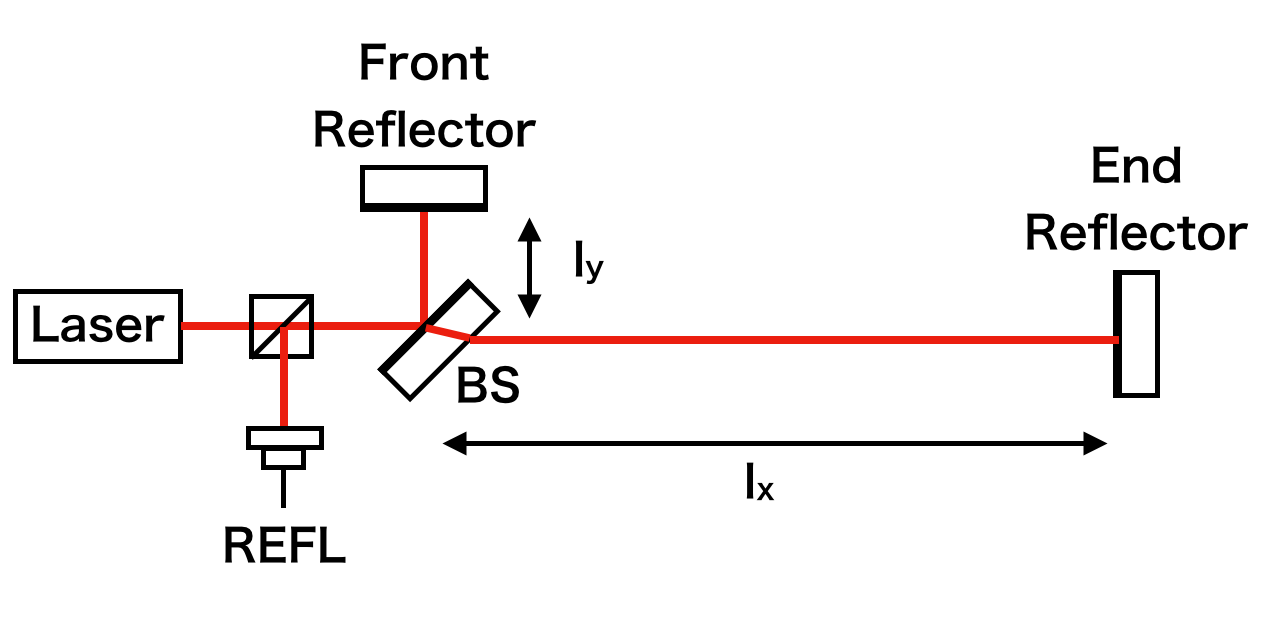
\includegraphics[width=10.0cm]{./img_chap4/img401.png}
  \caption{Asymmetric Michelson interferometer. Michelson interferometer which has two different arm length, $l_x\gg{l_y}$.} \label{img:img401}
\end{figure}

\cref{sec:12}で述べたとおり、マイケルソン干渉計の腕の差動成分${L_{-}}$と位相${\phi_{-}}$には、レーザーの波長を$\lambda$とすれば、${\phi}_{-} = 4\pi\frac{{L_{-}}}{\lambda}$の関係があるので、それらの微小変化には
\begin{eqnarray}  
  \left|\Delta \phi_{-}\right| = \frac{4\pi{L_{-}}}{\lambda}\left( \left|\frac{\Delta L_{-}}{L_{-}}\right| + \left|\frac{\Delta f}{f}\right|\right) \label{eq:eq400}
\end{eqnarray}
の関係がある。なお、$f$はレーザーの周波数であり、 $\Delta{\lambda}/\lambda = \Delta{f}/f$の関係をつかった。

ここで、2つの腕の長さ$L_{\mathrm{x}},\,L_{\mathrm{y}}$が十分に非対称、つまり$L_{\mathrm{x}} \gg L_{\mathrm{y}}$の場合を考える。また短い方の腕の長さ$L_{\mathrm{y}}$の変動が無視できるとすると、腕の差動成分は$\L_{-}\sim{L_{\mathrm{x}}}$と表すことができる。したがって、Eq.(\ref{eq:eq400})は、X腕のひずみ$h=\Delta{L_{\mathrm{x}}}/L_{\mathrm{x}}$をつかって
\begin{eqnarray}  
  \left|\Delta \phi_{-}\right| = \frac{4\pi{L_{\mathrm{x}}}}{\lambda}\left( \left|h\right|  + \left|\frac{\Delta f}{f}\right|\right) \label{eq:eq400_a}
\end{eqnarray}
となる。つまり非対称マイケルソン干渉計の場合、周波数ゆらぎ$|\Delta{f}/f|$はそのままひずみ計速のノイズとなる。

\subsection{Seismic Strain Response}
In order to calculate the response from the seismic strain to the optical phase of the GIF interferometer, the same as the Fig.(\ref{img:img310}), it is assumed that the plane seismic waves which displacement $u(t,x)$ is represented as $u(t,x)=u_0e^{i(\omega{t}-kx)}$ with angular frequency of $\omega$ and wave number of $k$, which propagates along with the direction of the baseline of the strainmeter (right direction in this figure). First, because the length fluctuation between two mirrors sparated with $L$ can be expressed as 
\begin{eqnarray} 
  \Delta{L(t)} &\equiv& u(t,0) - u(t,L) \\
  &=& u(t,0) - u(t-\tau,0), \label{eq:eq403}
\end{eqnarray}
where $\tau=L/v$ is the time delay, the transfer function from the displacement to the length fluctuation is given by Laplace transform as
\begin{eqnarray} \label{eq:eq404}
  H_{\mathrm{disp}}(s) \equiv \frac{\Delta{L(s)}}{u(s)} = \frac{u(s)\left[ 1-\exp(-\tau{s}) \right]}{u(s)} = 1 - \exp(-\tau{s})
\end{eqnarray}
Moreover, because the strain amplitude $\epsilon{(x,t)}$ is defined as $\epsilon{(x,t)}\equiv\frac{du}{dx}$, the seismic strain is represented as 
\begin{eqnarray} 
  \epsilon{(x,t)} \equiv \frac{du}{dx} = \frac{du}{dt} \frac{dt}{dx} =  \frac{du}{dt} \frac{1}{v} \label{eq:eq406}
\end{eqnarray}
Therefore, similarly, the transfer function from the seismic strain to the displacement is given  as
\begin{eqnarray} \label{eq:eq407}
  u(s) = \frac{v}{s} \epsilon(s).
\end{eqnarray}
Finary, because the transfer function from the length change of the baseline to the optical phase is given as $4\pi/{\lambda_{\mathrm{opt}}}$, the transfer function from the seismic strain to the optical phase is represented as 
\begin{eqnarray} \label{eq:eq407}
  H_{\mathrm{strain}}(s) = 4\pi\frac{1}{\lambda_{\mathrm{opt}}} \left[1 - \exp(-\tau{s}) \right]\frac{v}{s}.
\end{eqnarray}
Here, as a summary of these transfer function, these are related with each other as shown in Fig.(\ref{img:img411}). 

\begin{figure}[h]
  \centering
  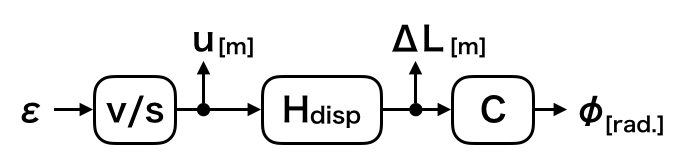
\includegraphics[width=10.0cm]{./img_chap4/img411.png}
  \caption{The response from seismic strain to optical phase. $\epsilon$ is the seismic strain, $u$ is the displacement, $\Delta{L}$ is the length change of the X-arm baseline, and $\phi$ is the optical phase of the GIF interferometer. $C$ is the optical gain of the GIF interferometer given in Eq.(\ref{eq:eq401}). $H_{\mathrm{disp}}$ is the transfer function from the displacement to the length change given in Eq.(\ref{eq:eq404}). $v/s$ is the transfer function from the seismic strain to the displacement given in Eq.(\ref{eq:eq406}). } \label{img:img411}
\end{figure}


Eq.(\ref{eq:eq407})で表される、基線長の異なる2つのMichelson干渉計のひずみから位相への伝達関数のボード図をFig.\ref{img:img411_a}に示す。長さが倍になるとDCでのゲインも2倍になる。コーナー周波数$f_0\equiv \frac{1}{\tau}$は
\begin{eqnarray}
  f_0 = \frac{v}{L}
\end{eqnarray}
で表せるので、長さが二倍になるとコーナー周波数は半分になり、帯域が減ることもわかる。基線長が$1500\,\mathrm{m}$のGIFの場合、弾性波速度を$5.5\,\mathrm{km}$とすれば、コーナー周波数は$f_0\sim3.7\,\mathrm{Hz}$である。つまりそれ以下の帯域ではGIFは歪に対して平坦な応答を示す。

\begin{figure}[p]
  \begin{center}
    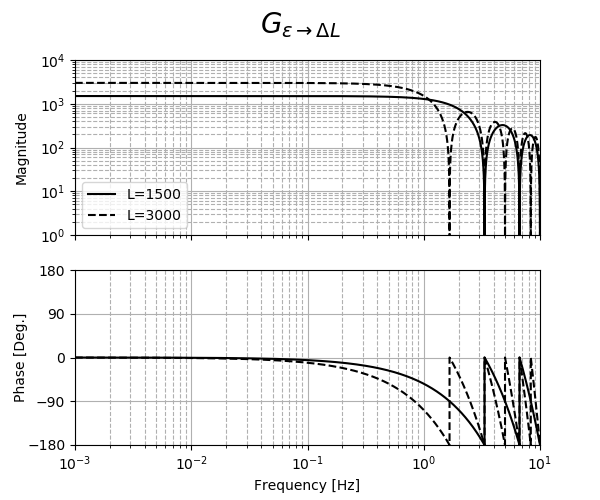
\includegraphics[width=13.0cm]{./img_chap4/img412.png}
    \caption{Compasison of the transfer function from strain of the baseline $\epsilon$ to the length change of that $\Delta{L}$ in the different baseline length. $3000\,\mathrm{m}$ の基線長ではその半分の$1500\,\mathrm{Hz}$よりも、DCゲインは二倍大きい一方で、コーナー周波数は \color{red}{A} になり帯域が減る。また、周波数が \color{red}{B} の条件を満たすとき、ゲインはゼロになる。なぜならば、このときひずみは基線を同相で動かし、基線長伸縮として現れないためである。}\label{img:img411_a}
  \end{center}
\end{figure}

\subsection{Noise}
\subsubsection{Frequency Noise}
先述したように、GIFのような1500mと70cmの腕を持つ非対称マイケルソン干渉計は、腕の同相雑音除去が効かない。周波数ノイズは
\begin{eqnarray}
  h = \frac{\Delta{f}}{f} \sim 7\times10^{-13} [\mathrm{1/\mathrm{Hz}}]
\end{eqnarray}
になる\cite{araya2017design}。

\subsubsection{Residual Gas Noise}
Bcause residual gas fluctuates the optical path, length measured by interferometer is also fluctuates. The opttical path $L_{\mathrm{opt}}$ is given by $L_{\mathrm{opt}}=nL$, where $L$ is the length of the baseline and $n$ is the refraction index in the optical path relative to the path in the vacuum. Under the pressure of $p$ in vacuum, the index $n$ is approximated as $n = 1 + c_0(p/p_0)$, where $c_0$ denotes the relattive refractive index, $p_0$ is pressure in standard air at 1 atm. The apparent strain due to the residual pressure is given as \cite{ciddor1996refractive};
\begin{eqnarray}
  h = (L_{\mathrm{opt}}-L)/L = c_0(p/p_0) \sim 3\times10^{-9} p.
\end{eqnarray}
In order to maintain the strain sensitivity; $3\times10^{-13}$, the vacuum pressure should be below $1\times10^{-4}\,[\mathrm{Pa}]$. However, actual vacuum pressure is $1\times10^{-2}\,[\mathrm{Pa}]$, then strain is $\sim\times10^{-12}$.

\subsubsection{Thermal fluctuation of the reference arm }
AAAAAAA


\section{Optics} %光学系
\subsection{Gaussian Beam}
理想的なレーザー光は$\mathrm{TEM}_{00}$と呼ばれる空間モードをもち、電場の位相は距離に応じて変化する。この空間モードをもつビームのことをガウシアンビームと呼ぶ。このガウシアンビームが$z$軸に伝搬する場合を考える。この電場は
\begin{eqnarray}
  u(x, y, z)=\sqrt{\frac{2}{\pi{w^2(z)}}} \exp \left(i\zeta(z)-\mathrm{i} k \frac{x^{2} +y^{2}}{2 R(z)}-i\frac{2\pi}{\lambda}z\right)
  \exp \left(-\frac{x^{2}+y^{2}}{w^{2}(z)}\right)  \label{eq:eq415}
\end{eqnarray}
とかける\cite{bond2016interferometer,svelto1998principles}。ここで、$\lambda,\,w_0$はそれぞれレーザーの波長、$z=0$でのビーム径である。また
\begin{eqnarray}
  z_0 &=& \frac{\pi{w^2_0}}{\lambda} \\ \label{eq:eq415_a}
  w(z) &=& w_0\sqrt{1+\left(\frac{z}{z_0}\right)^2}, \\ \label{eq:eq415_b}
  R(z) &=& z\left[1+\left(\frac{z_0}{z}\right)^2\right],\\ \label{eq:eq415_c}
  \phi(z) &=& \arctan\left(\frac{z}{z_0}\right) \label{eq:eq415_d}
\end{eqnarray}
はそれぞれ、Reyliegh length、$z$でのビーム径、曲率、Gouy位相である。このときEq.(\ref{eq:415})から、Fig.\ref{img:img415a}にしめすように、ガウシアンビームのパワー$P=|u^2|$はガウス分布をもつことがわかる。さらにビーム径はビーム強度が$1/e^2$になるときの半径とわかる。
\begin{figure}[p]
  \begin{minipage}{14cm}
    \centering    
    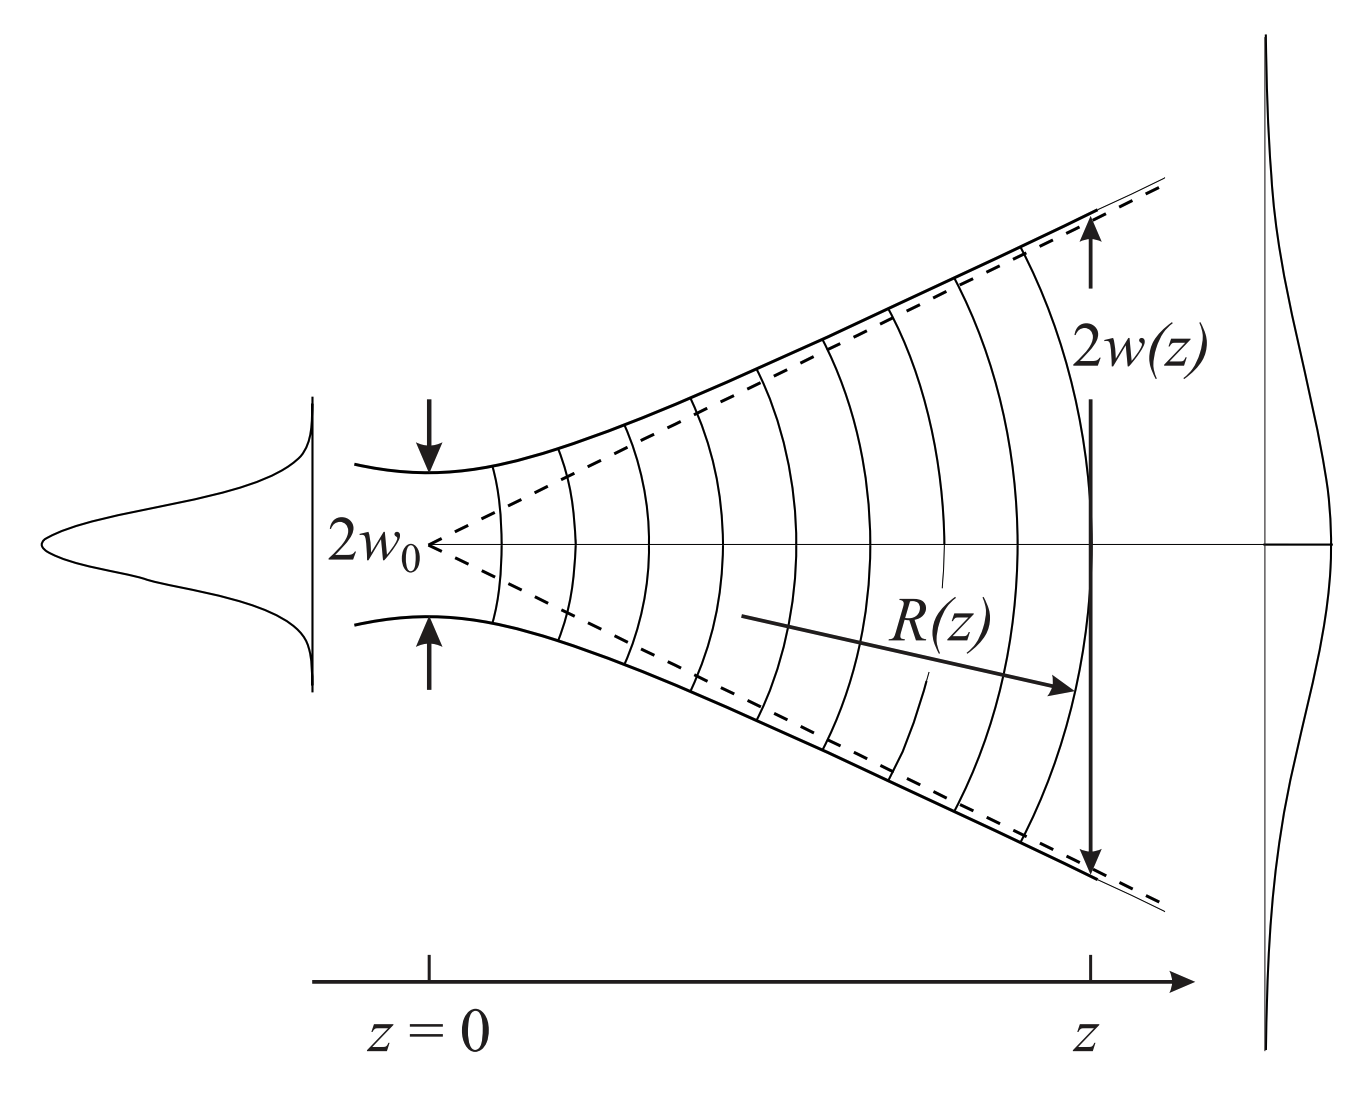
\includegraphics[width=8cm]{./img_chap4/img415a.png}
    \subcaption{Evolution of a Gaussian beam propagating along the z-axis\cite{riehle2006frequency}}{$w_0$ denotes a beam radius at beam weist, where $z=0$. $w(z)$ and $R(z)$ are the beam radius and curvature at $z$. Gouy phase is not shown in here.}\label{img:img415a}
  \end{minipage}\\
  \begin{minipage}{14cm}
    \centering        
    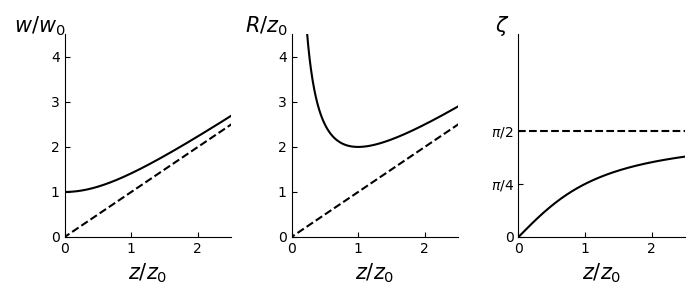
\includegraphics[width=14cm]{./img_chap4/img415.png}
    \subcaption{Beam prifile}{(left) Beam radius normalized by $w_0$ as a function of $z/z_0$, where $z_0$ is Rayleigh length. (Middle) Beam curvature normalized by $z_0$. (right) Gouy phase.}\label{img:img415}    
  \end{minipage}
  \caption{Gaussian beam.}
\end{figure}


ガウシアンビームを特徴づける$z$の関数であるパラメータEq.(\ref{eq:eq415_b,eq:eq415_c,eq:eq415_d})をFig.{\ref{img:img415}}に示す。$z=0$のとき、ビーム径は最も小さくEq.(\ref{eq:eq415})の位相は0であるため、ガウシアンビームは平面波とみなせる。一方で、$z\gg{z_0}$のときレーザー光源は点光源とみなせ、球面波としてふるまう。


\subsection{Reflector Design}
リフレクタの大きさを最小限にするために、GIFの干渉計はエンドミラーでビーム直径が最も小さくなるビームウエストがくるようにしている。この場合、ビームウエスト$w_0$を小さくしたいが、小さくしすぎると$L=1500\,\mathrm{m}$離れたBSとフロントリフレクタで大きくなるので、できるだけフロントでのビーム径$w(L)$はエンドのビーム径$w_0$に対してできる限り小さくしたい。つまりこれを式で表すと、
\begin{eqnarray}
  \argmin_{w_0} \left[w_0\times\frac{w(L)}{w_0}\right] \label{eq:eq415_e}
\end{eqnarray}
となるような$w_0$を探せばよい。Eq.(\ref{eq:eq415_b})をEq.(\ref{eq:eq415_e})に代入して解けば
\begin{eqnarray}
  w_0 = \sqrt{\frac{{L\lambda}}{\pi}}
\end{eqnarray}
を得る。つまりビームウエストサイズ$w_0=\sqrt{{1500\,\mathrm{[m]}}\times 532\,\,\mathrm{[nm]}/\pi} = 16\,\mathrm{mm}$となる。このときのフロントリフレクタでのビーム径は$w(L)=\sqrt{2}{w_0}$になる。ちなみに、リフレクタの大きさはフロントリフレクタでのビーム径の3倍の大きさを往復できるようにするには、最低限必要なリフレクタの aperture diameter は$2\times3\times\sqrt{2}w_0\sim270\,\mathrm{mm}$となる。

\subsection{Input Output Optics}
レーザー光源から出射されたビームを適当な大きさにして干渉計へ入射するために、input output optics と呼ばれる光学系を構築している。Fig(\ref{img:img416})にGIFのinput output optics と干渉計を示す。光源からの出射ビームは、エンドリフレクタの位置Aでビームウエストになるように、コリメータ(1)とステアリングミラー(2)、凹面鏡(3)を経てBSへと入射される。2つのリフレクタから反射してきたビームは地点Bで再結合し、2つ目の凹面鏡とコリメータ(4)をへてPDに入射する。これらopticsの調整をおこない干渉信号を得ている\cite{miyo2017baseline}。

\begin{figure}[h]
  \begin{center}   
    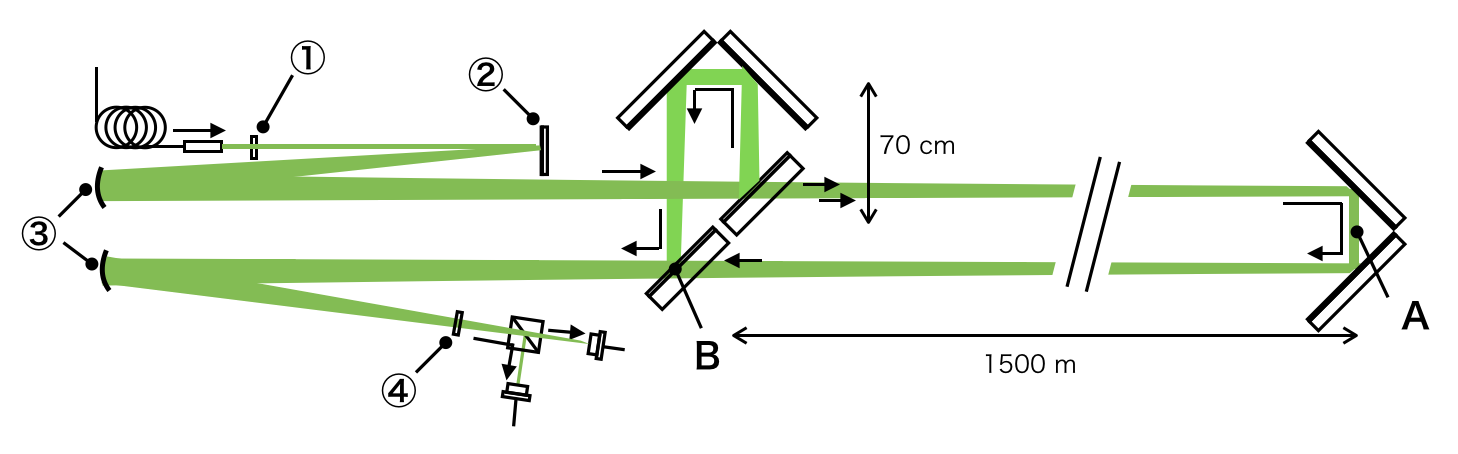
\includegraphics[width=14cm]{./img_chap4/img416.png}
    \caption{Schematic optics layout}{(1) A collimator lens for input beam. (2) A flat mirror for steering mirror. (3) Two concave mirrors with a radius of curvature of $9.8\,\mathrm{m}$ for mode matching. (4) A collimator lens for output beam. The waist of the beam is at the end reflector at point A. Two reflected on the reflectors are combined at point B.}\label{img:img416}
  \end{center}
\end{figure}


\subsection{Core Optics}
The core optics of the Michelson interferometer are composed of two reflectors and beam splitter (BS). 

\begin{figure}[h]
  \begin{minipage}[b]{7cm}
    \begin{center}   
      %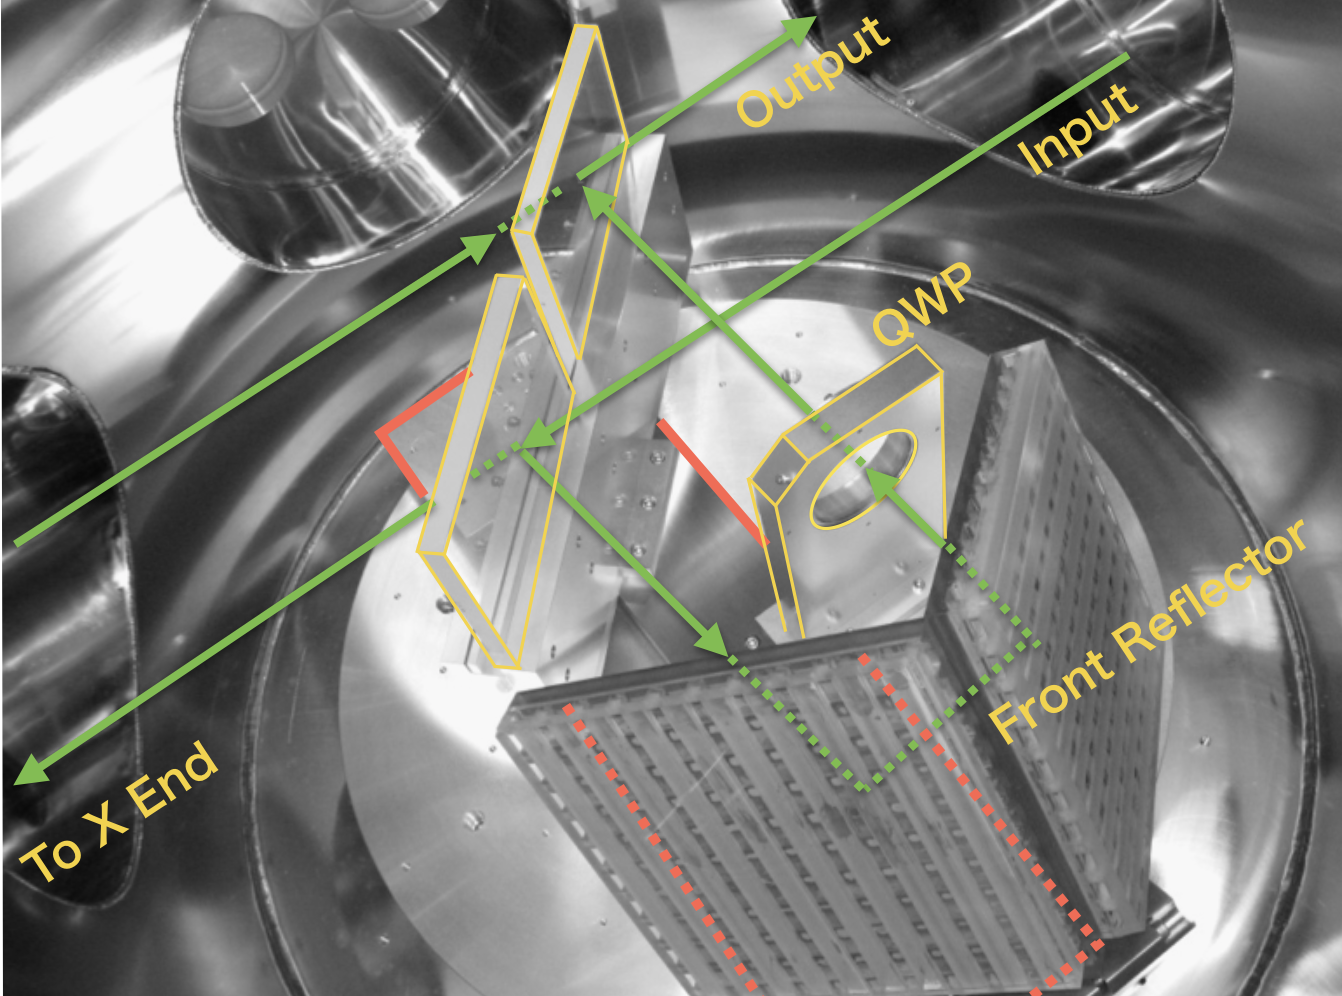
\includegraphics[width=7cm]{./img_chap4/img418.png} % ファイル重い
      
\includegraphics[width=7cm]{./img.png}
      \subcaption{Core optics in the front vacuum chamber. }\label{img:img418}
    \end{center}
  \end{minipage}\hspace{0.1cm}
  \begin{minipage}[b]{7cm}
    \begin{center}   
      %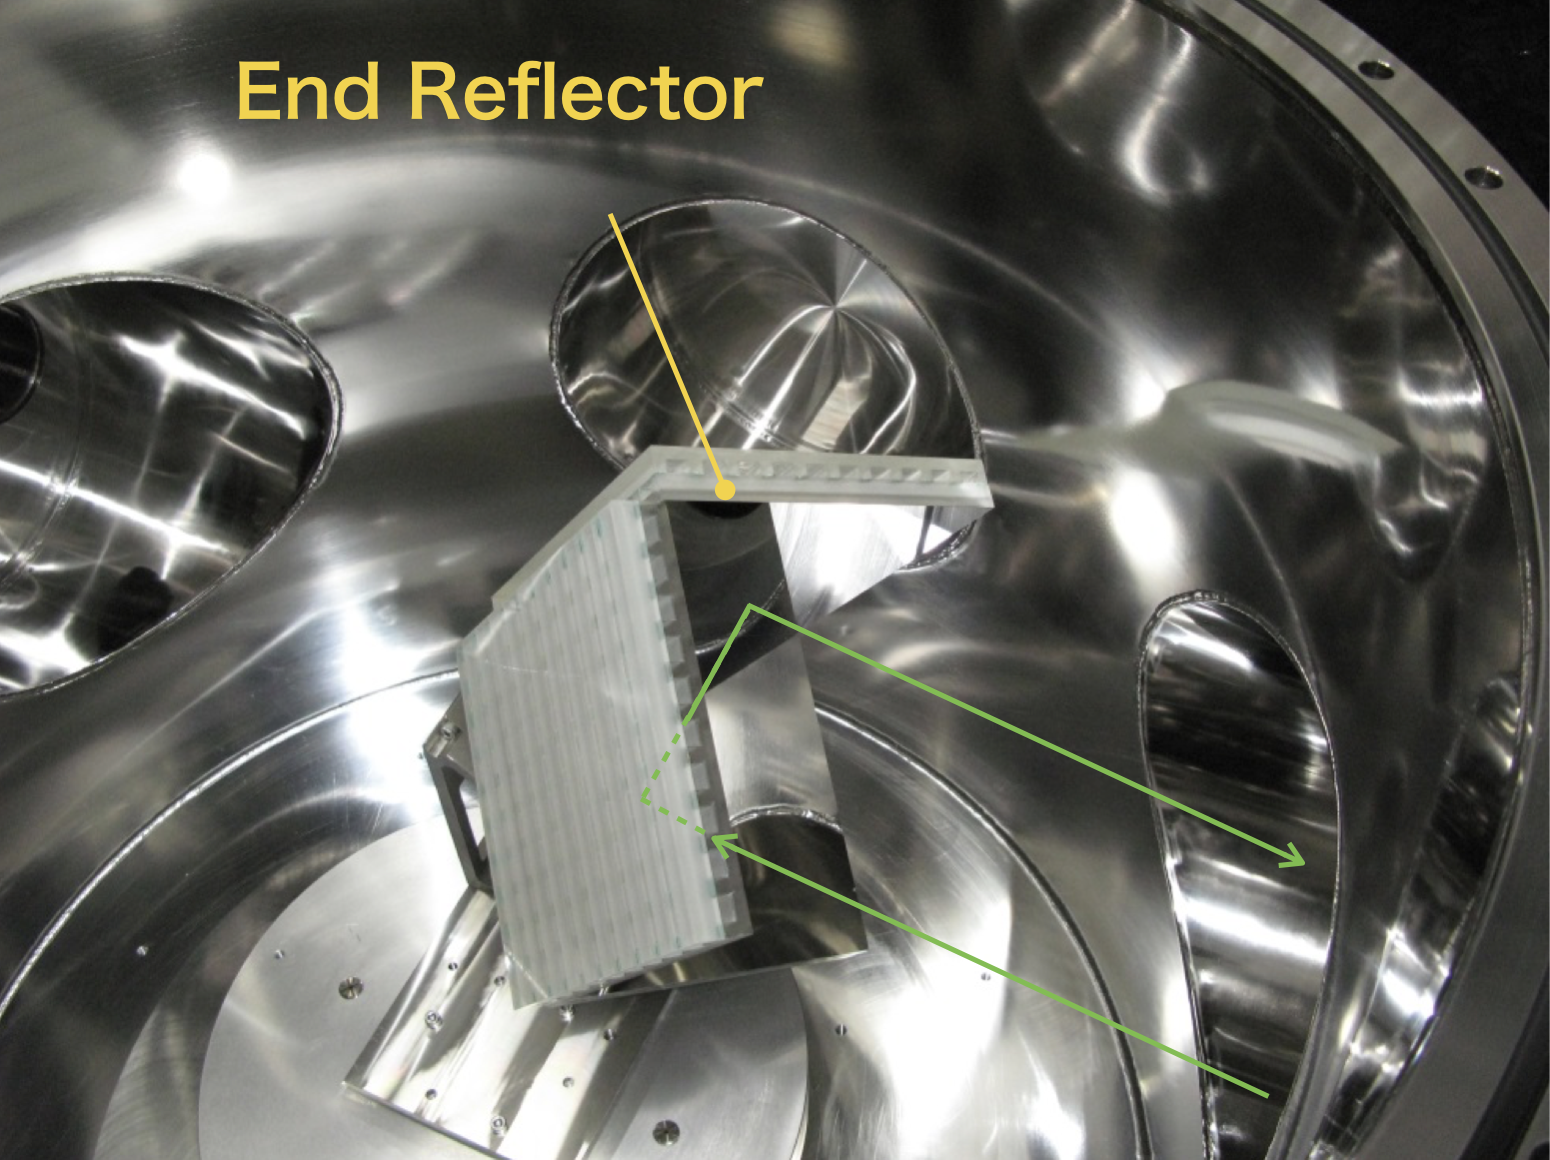
\includegraphics[width=7cm]{./img_chap4/img419.png} %ファイル重い
      
\includegraphics[width=7cm]{./img.png}      
      \subcaption{Core optics in the end vacuum chamber. }\label{img:img419}
    \end{center}
  \end{minipage}
  \caption{}  
\end{figure}


\subsection{Frequency Stabilized Laser}
Because GIF is an asymmetric Michelson interferometer, the frequency stability of the laser would limit the sensitivity of the strain, and we use the frequency stabilized laser, which is stabilized the laser frequency to the iodine absorption line \cite{araya2002iodine}. The control diagram of the frequency stabilization system is shown in Fig.\ref{img:img417}. このシステムはヨウ素分子の吸収スペクトル線の周波数とレーザーの周波数との差を利用したフィードバック制御である。エラー信号は、ポンプ光とプローブ光をつかったドップラーフリーな吸収線信号\cite{snyder1980high}をPDH法をつかって取得する。

\begin{figure}[h]
  \begin{center}   
    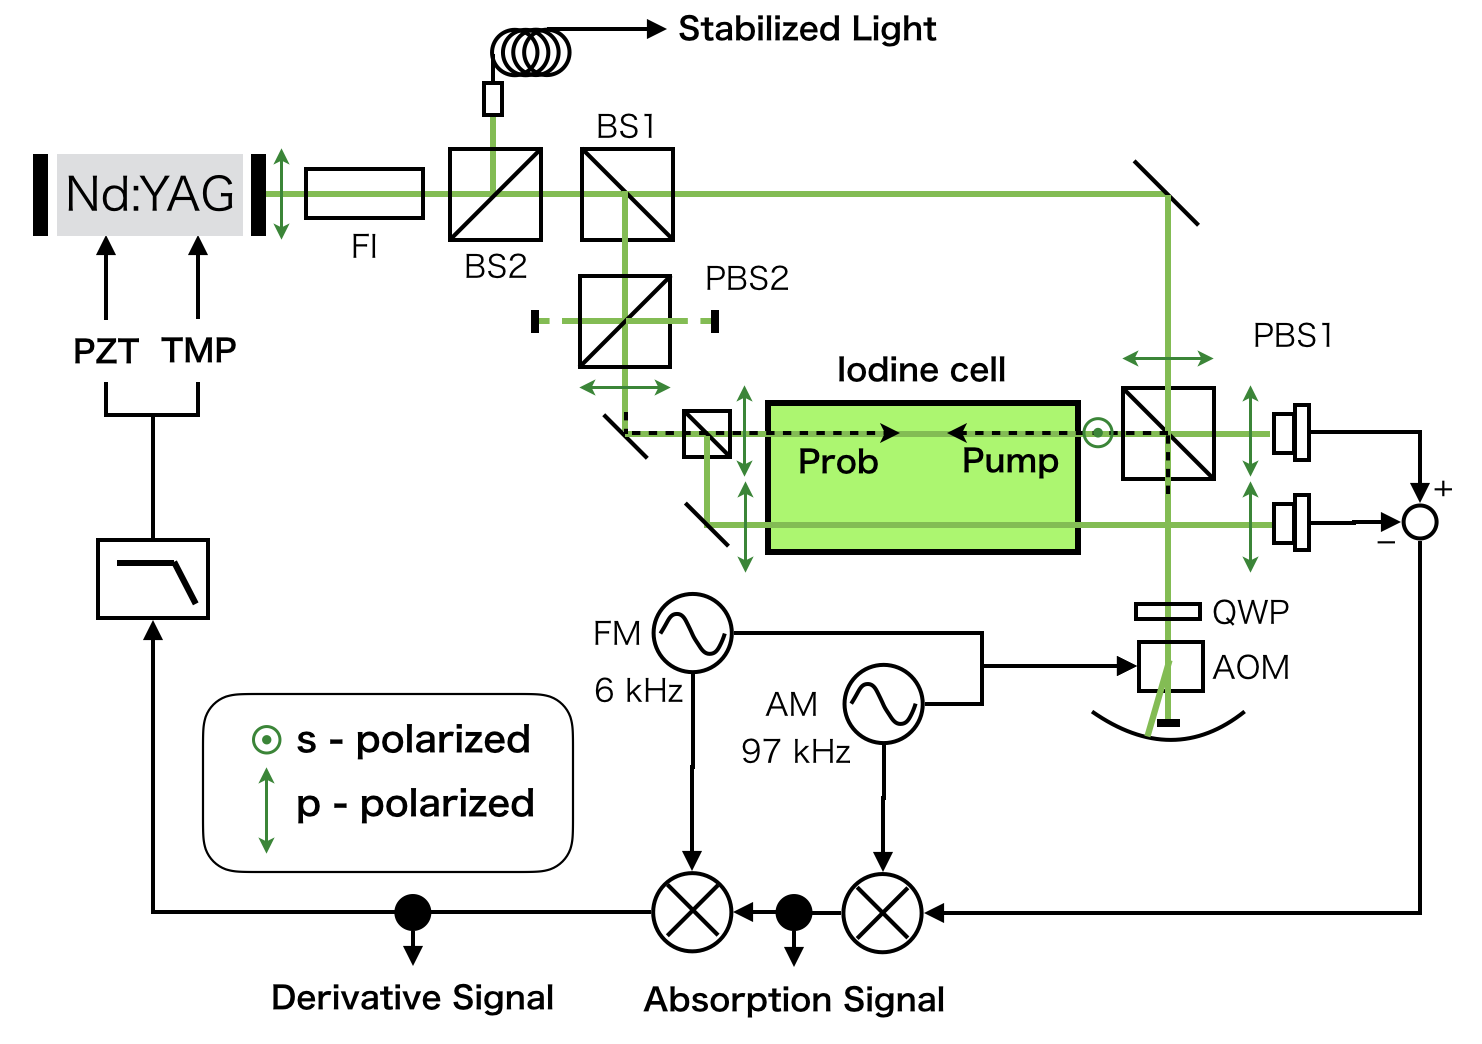
\includegraphics[width=12cm]{./img_chap4/img417.png}
    \caption{Schematic diagram of the frequency-stabilization system of the GIF main laser.}\label{img:img417}
  \end{center}
\end{figure}

\section{Realtime Signal  Aquisition System} \label{sec:sec33}
\subsection{Quadrature Phase Fringe Detection}
\begin{figure}[h]
  \begin{center}
    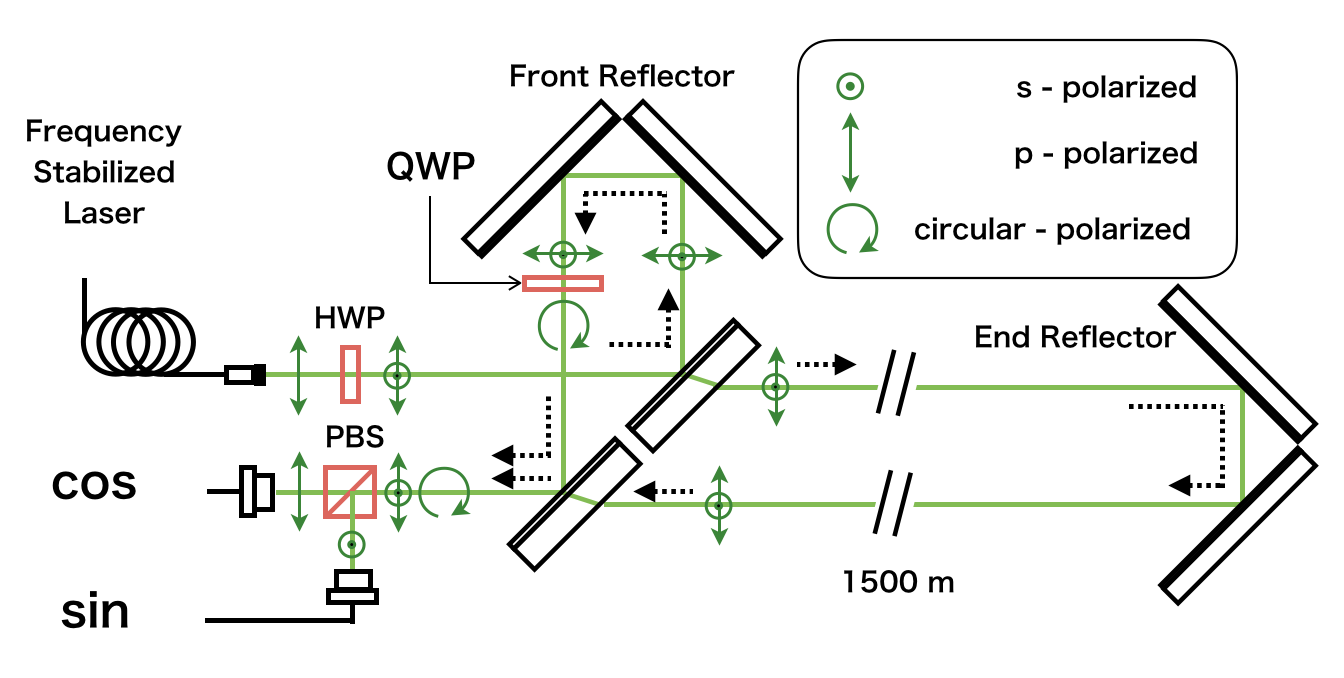
\includegraphics[width=13.0cm]{./img_chap4/img413.png}
    \caption{Quadrature interferometer used in the GIF strainmeter. A half-wave plate (HWP) produces a p-polarization and s-polarization. A quator-wave plate (QWP) delay the optical phase of the s-polarized light with 90 degree against to the another. As a result, one can obtain the quadrature phase fringe.}\label{img:img413}
  \end{center}
\end{figure}

We use the quadrature phase fringe detection to measure the length change of the baseline with wide dynamic range \cite{bobroff1993recent}. The optical layout for the detection is shown in Fig.(\ref{img:img413}).

The quadrature phase fringes are detected by two photo detectors, these can be represented as
\begin{eqnarray}
  x(t) &=& x_0 + a \sin(\phi(t)+\phi_0), \\
  y(t) &=& y_0 + b \cos(\phi(t)),
\end{eqnarray}
where $x$ and $y$ are the two voltage outputs from the detectors, $a$ and $b$ are the amplitudes of these fringe signals, $x_0$ and $y_0$ are the offsets, $\phi$ is optical phase, and $\phi_0$ is the phase offsets from imperfections \cite{zumberge2004resolving}.
このとき、位相角$\phi$は
\begin{eqnarray}
  \tan{\phi(t)} = \frac{1}{{\cos(\phi_0)}} \left(\displaystyle{\frac{b}{a}\frac{x(t)-x_0}{y(t)-y_0}-\sin(\phi_0)}\right)
\end{eqnarray}
で表される。つまりある時刻$t$のときに、パラメーター$x_0,\,y_0,\,a,\,b,\,\phi_0$が与えられれば、そのときの位相$\phi(t)$は求まる。

\subsection{Realtime Data Processing}
KAGRAのデジタルシステムをつかってリアルタイムで楕円パラメータを取得する。KAGRAのデジタルシステムでは

\cite{bork2001overview}


GIFからの2つの干渉信号を

Fig.\ref{img:img420}にひずみ変換のMatlabのSimlinkモデルを示す。

\begin{figure}[h]
  \centering
  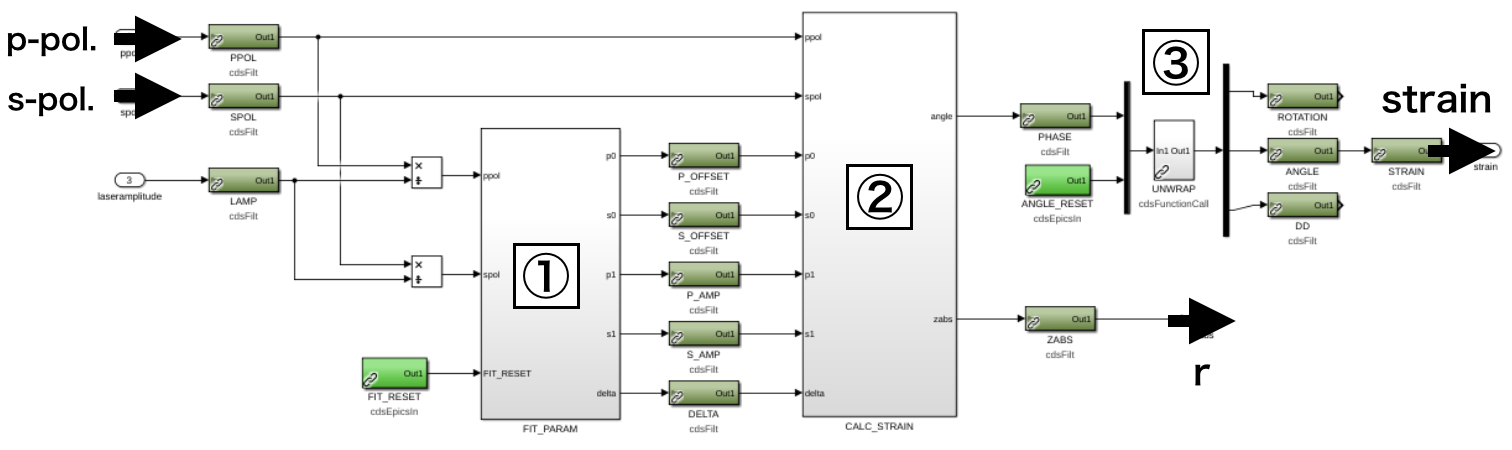
\includegraphics[width=15.0cm]{./img_chap4/img420.png}
  \caption{}\label{img:img420}
\end{figure}



\section{Summary of the Chapter} %章のまとめ
本章で述べたパラメータを表にまとめる。
